\section{Energie als Produktionsfaktor}

\textbf{Endkundenmarkt:} 
\begin{itemize}
	\item Liberalisierung der Strommärkte: freie Wahl der Energielieferanten
	\item Endkunden können aus über 1200 unterschiedlichen Stromlieferanten deutschlandweit wählen
\end{itemize}
\bigskip
\textbf{Endkundentypen:}
\begin{itemize}
	\item \textbf{SLP Kunden}:
	\begin{itemize}
		\item Privathaushalte/Gewerbekunden mit Jahresstromverbrauch $\leq$ 100.000 kWh
		\item Ohne registrierte Leistungsmessung: Lastgang wird mittels Standardlastprofil ermittelt
	\end{itemize}
	\pagebreak
	\item \textbf{RLM Kunden}:
	\begin{itemize}
		\item Industriekunden und große Unternehmen
		\item Registrierende Leistungsmessung ab Jahresstromverbrauch $>$ 100.000 kWh
	\end{itemize}
\end{itemize}
\bigskip
\textbf{Lastganglinie:} Darstellung der Leistungsaufnahme von Abnehmern über einen bestimmten Zeitraum $\rightarrow$ \textit{s. \textbf{H0/G0-Profile} VL 3, F7-8}

\textbf{Strompreis für einen Haushalt:} ca. 40 ct/kWh, Tendenz steigend

\textbf{Prosumer:} Sowohl Producer als auch Consumer, z.B. durch PV-Anlage $\rightarrow$ Transformation des zentralen Stromsystems zu dezentralem Stromsystem

\textbf{Eigenverbrauchsquote:} Anteil der lokalen Erzeugung, der selbst verbraucht wird

\textbf{Autarkiegrad:} Anteil der gesamten jährliche Stromnachfragen die durch eigene Erzeugung gedeckt wird

\textbf{Netzparität:} Zeitpunkt, ab dem die Kosten für Strom aus erneuerbaren Energien genauso hoch sind wir für Strom, der aus dem Netz bezogen wird

\begin{center}
	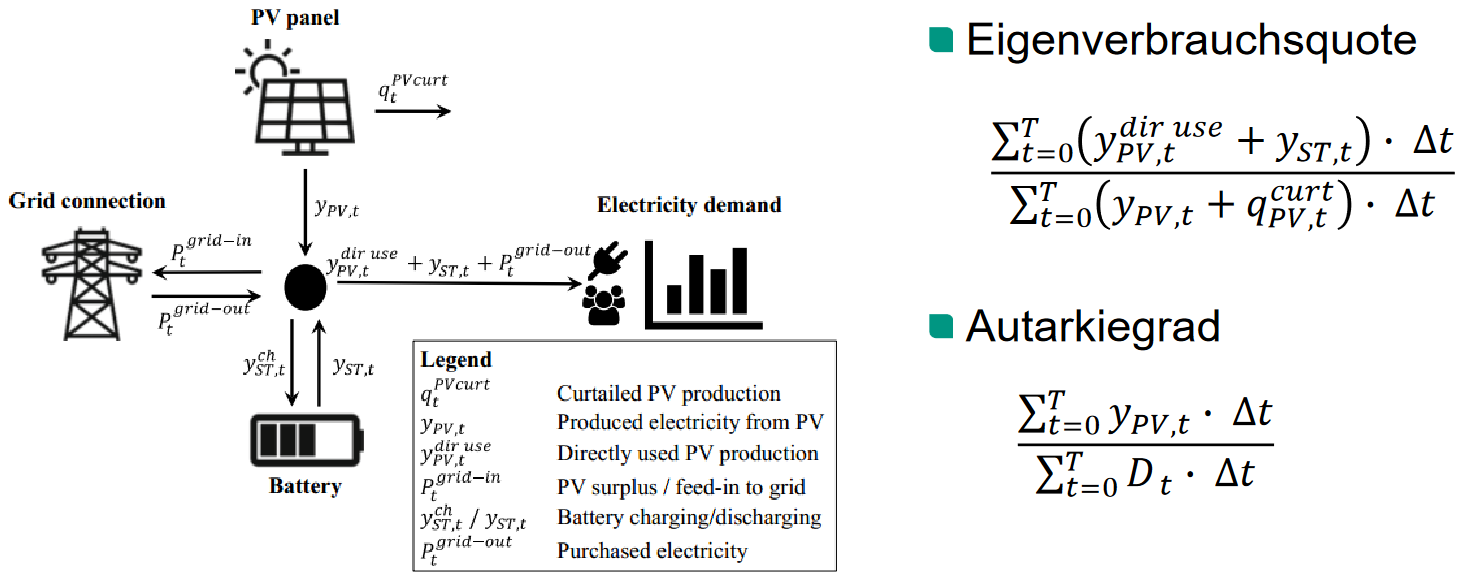
\includegraphics[width=0.8\textwidth]{images/ea.png}
\end{center}

\textbf{Smart-Meter:} Intelligente Messsysteme zur effizienten Steuerung des Stromverbrauchs entsprechend der volatilen Erzeugung

\textbf{Stromtarife:}
\begin{itemize}
	\item Zeitvariable Tarife: Time-of-use, Critical Peak Pricing, Real-Time-pricing
	\item Lastvariable Tarife
	\item Dynamische Tarife
\end{itemize}
\bigskip
\textbf{Energie in der Industrie:}
\begin{itemize}
	\item Mehr als ein Viertel des Energieverbrauchs in Deutschland entfällt auf die Industrie
	\item Erdgas und Strom sind wichtigste Energieträger in der Industrie
	\item Große regionale Unterschiede beim Energieverbrauch
	\item Größter Energieverbraucher: Chemische Industrie
\end{itemize}
\bigskip
\textbf{Bewertung der Produktionsprozesse hinsichtlich des Energieverbrauchs:}
\begin{itemize}
	\item Energieintensität $=$ Energieverbrauch pro Tag $/$ Stückzahl pro Tag
	\item Effizienzgrad $=$ Referenzwert $/$ gemessener Energieverbrauch
\end{itemize}
\bigskip
\textbf{Energiewertstrommethode:}
\begin{itemize}
	\item Methode zur Analyse der Energieeffizienz
	\item \textbf{Energiewertstromanalyse}: Aufnahme der Energieverbraucher mit den Verbrauchswerten, Ermittlung des Energieeinsparpotenzials
	\item \textbf{Energiewertstromdesign}: Gestaltung eines Soll-Konzepts anhand von Richtlinien (\textit{s. VL 3, F27}), Ableitung von Verbesserungsmaßnahmen
	\item \textbf{Umsetzung}: Umsetzung des Soll-Konzepts durch Maßnahmen
\end{itemize}

\textbf{Ziele der Energiewertstromanalyse:}
\begin{itemize}
	\item Kennzahlenbildung zur Effizienzbewertung
	\item Grundlage für die Optimierung des Energieeinsatzes
	\item Abschätzung der Energieeinsparpotenziale
	\item Identifikation der wesentlichen Energieverbrauchsarten
\end{itemize}